\documentclass[xcolor=svgnames,handout]{beamer}
\usepackage{alltt}
\usepackage{graphicx}
\usepackage[utf8]{inputenc}
\usepackage{pifont}  % checkmark sybmols
\usepackage{xspace}

\graphicspath{{figs/}}

\usetheme{bro}

\title{Bro Integrations:}
\subtitle{Some Misc. Bro Related Stuff}
\author{Jon Schipp, \small NCSA}
\institute{%
BroCon15 \\
MIT, Cambridge, Massachusetts
}
\date[]{}

\newcommand{\checked}{\textcolor{olive}{\ding{51}}\xspace}
\newcommand{\unchecked}{\textcolor{red}{\ding{55}}\xspace}

\begin{document}

\begin{frame}[plain]
  \titlepage
\end{frame}

\section{Integrations}

\begin{frame}[fragile]{}
  \begin{block}{Agenda}
    \begin{itemize}
      \item Outlining a few things I've worked on
    	\begin{itemize}
      		\item ISLET - Software that can be used for Bro training
      		\item Mal-dnssearch - Create Bro intel feeds from command-line
      		\item Sagan - Log analysis on Bro logs
      		\item Nagios - A plug-in to monitor your Bro cluster
    	\end{itemize}
    \end{itemize}
  \end{block}
\end{frame}

\begin{frame}{ISLET}
  \begin{block}{Isolated Scalable and Lightweight Environment for Training}
    \begin{itemize}
      \item Background
    	\begin{itemize}
		\item The brototype released at BroCon'14 as BroLive!
                \item Saw something greater and morphed into ISLET
    	\end{itemize}
      \item How?
    	\begin{itemize}
		\item Linux kernel has namespaces and control groups
    	        \begin{itemize}
		  \item Lightweight process virtualization
    	        \end{itemize}
		\item A container based solution for easy deployment
    	\end{itemize}
      \item Why?
    	\begin{itemize}
		\item Improve Bro training
    	        \begin{itemize}
		  \item Containers have millisecond startup times
		  \item Scalability - hundreds or thousands of users
		  \item VM's are slower, costlier, and larger
    	        \end{itemize}
    	\end{itemize}
    \end{itemize}
  \end{block}
\end{frame}

\begin{frame}{ISLET Cont.}
  \begin{itemize}
    \item \textbf{User Perspective:} Looks and feels like a Virtual Machine
    \item \textbf{User Perspective:} Only needs a remote access tool like a ssh client
    \item \textbf{Admin Perspective:} Deployment of ISLET is dead simple
  \end{itemize}
    \begin{exampleblock}{Deploying Bro with ISLET}
	\alert{\$ git clone http://github.com/ncsa/islet \&\& cd islet} \\
        \alert{\$ make bro-training}
    \end{exampleblock}
    \begin{exampleblock}{Use}
	\alert{\$ ssh demo@islet.server.org} \\
    \end{exampleblock}
    \item \textbf{Official Image:} https://registry.hub.docker.com/u/broplatform/brolive/
\end{frame}

\begin{frame}{ISLET Cont.}
  \begin{itemize}
    \item Published a paper on ISLET using Bro
  	\begin{itemize}
		\item Substantiated container startup times with shell
		\item Compared costs using virtual machines and containers
		\item Benchmarked concurrent containers and simulated Bro users
	\end{itemize}
  \end{itemize}
  \begin{exampleblock}{Retrieve Paper}
	\alert{\$ curl http://jonschipp.com/islet/islet-paper.pdf > islet-paper.pdf }
    \end{exampleblock}
\end{frame}

\begin{frame}{ISLET/Bro Benchmark}
  \begin{itemize}
    \item Simulated Bro training benchmark
    \begin{itemize}
      \item Program execution/response time is good indicator for training software
      \item EC2 c4.4xlarge(16CPU,30GB RAM) handles 100+ \textcolor{blue}{overly} active users
    \end{itemize}
      \item Anecdotally, 100+ users in the wild doing real training
  \end{itemize}
  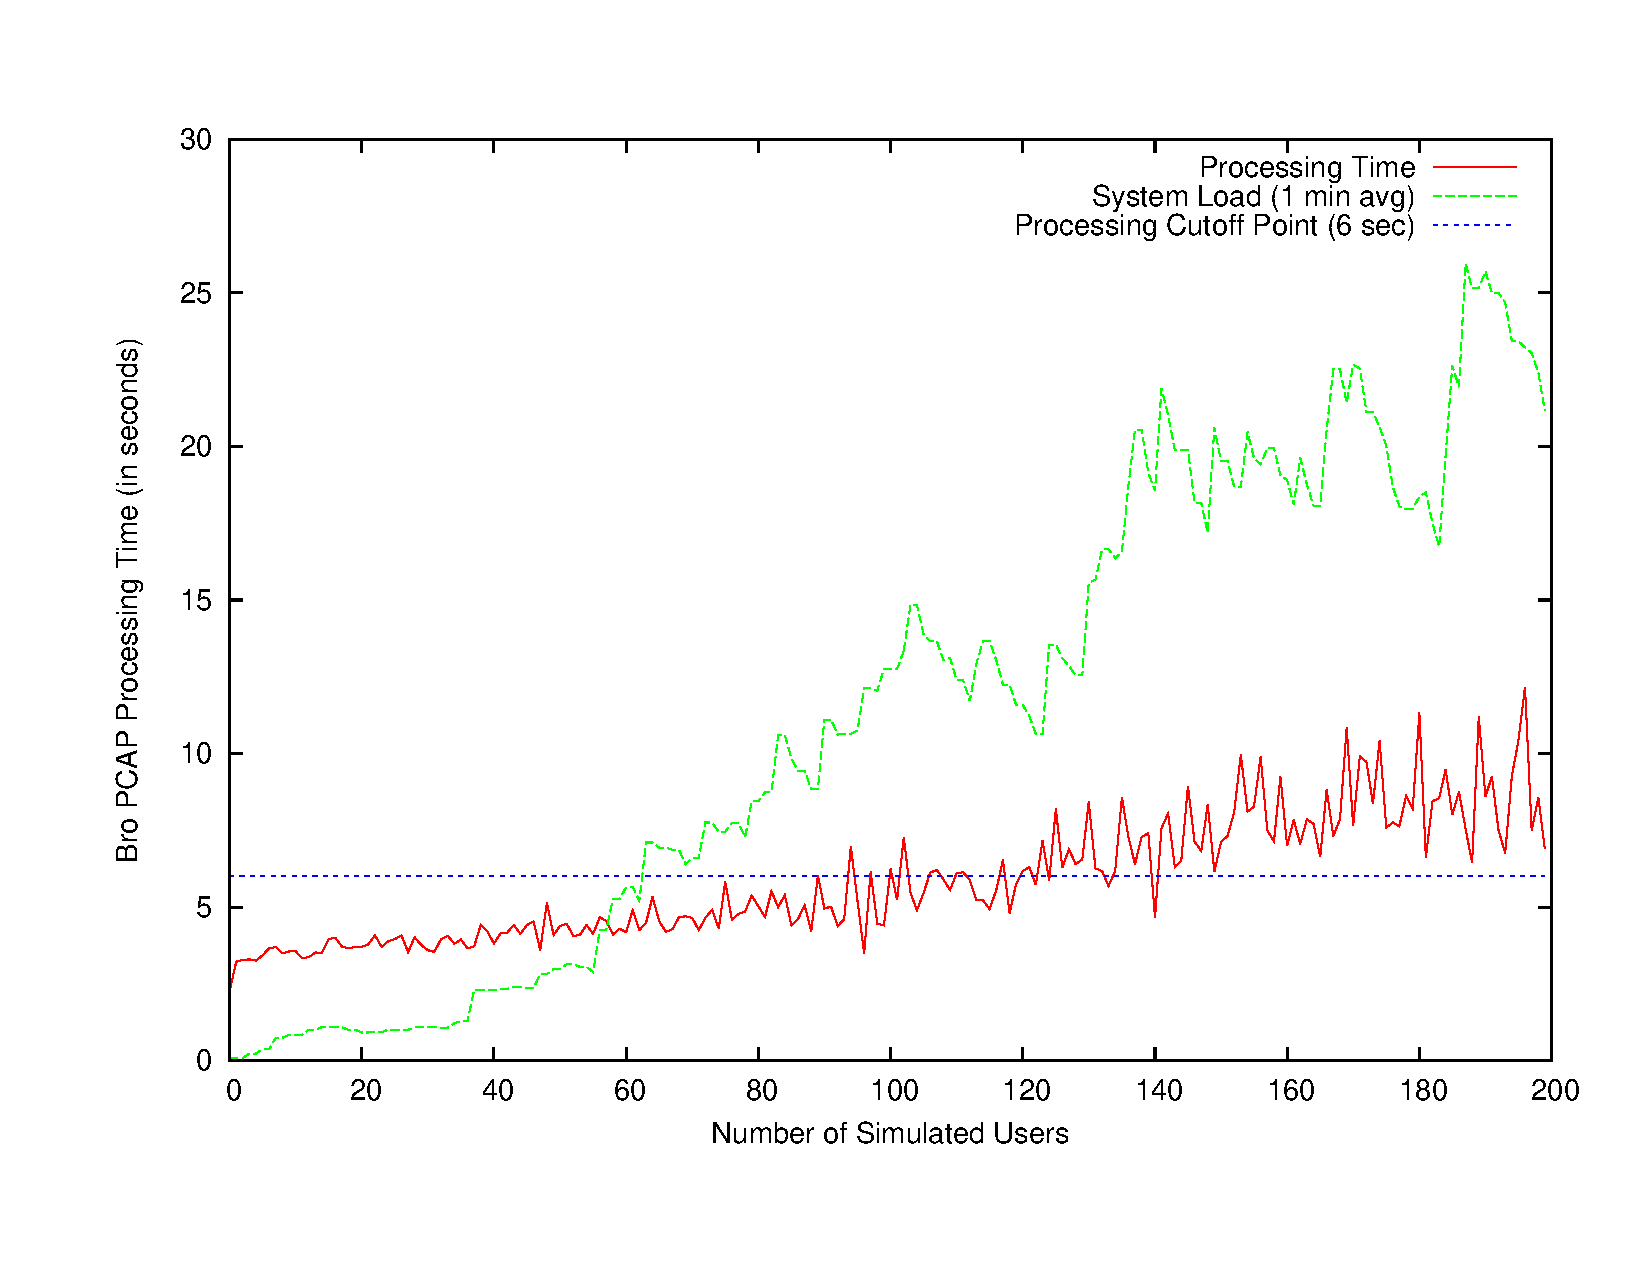
\includegraphics[height=.75\textheight,width=1\textwidth]{container_simulation.pdf}
  %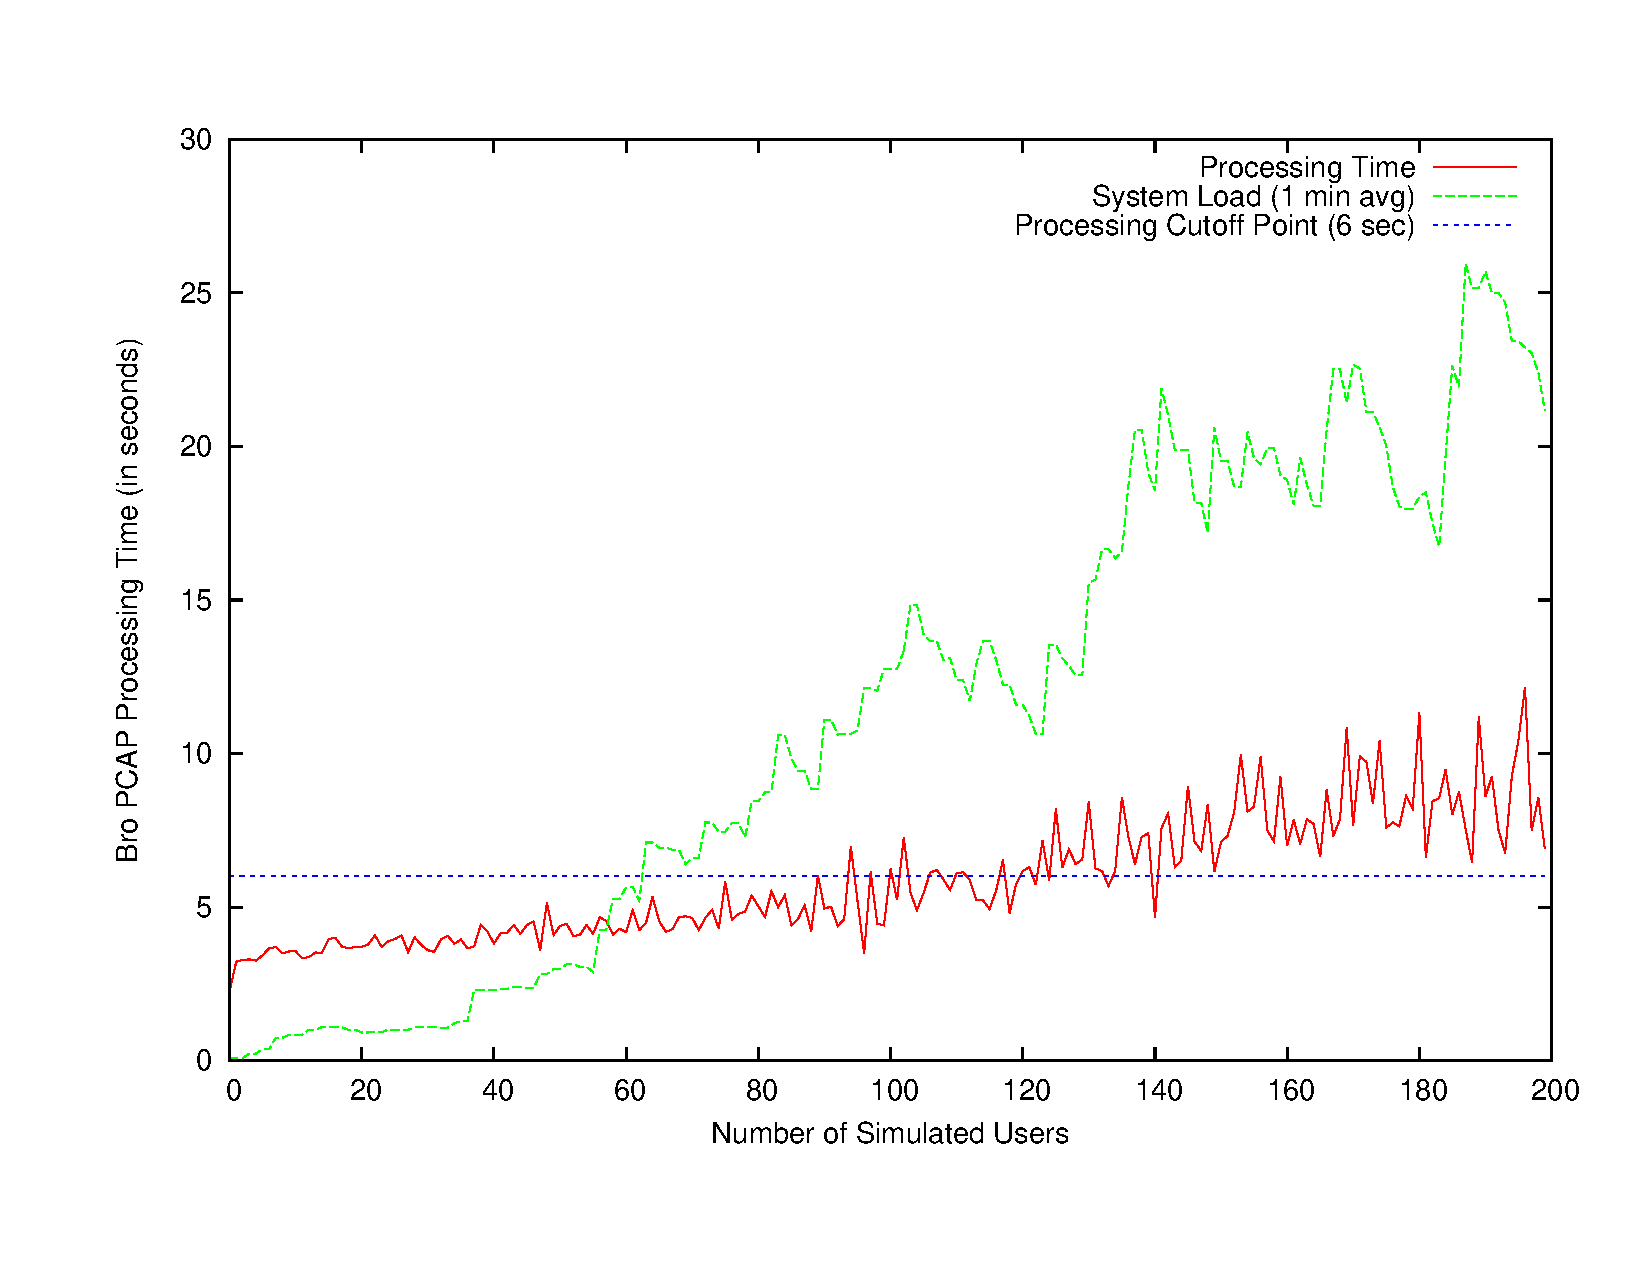
\includegraphics[scale=0.33]{container_simulation.pdf}
\end{frame}

\begin{frame}{Mal-dnssearch}
  \begin{block}{Intel tool}
    \begin{itemize}
      \item What?
    	\begin{itemize}
		\item Command-line intelligence pulling and matching script
		\item Pulls existing feeds and supports many input logs e.g. PCAP, bind, Bro
		\item Can generate data for Bro Intelligence Framework
	\end{itemize}
	\item Why?
    	\begin{itemize}
		\item While writing the Bro and Intelligence Data post for the
                  Bro blog I was looking for quick and easy way to test and
                  create intel feeds.
	\end{itemize}
	\item How?
    	\begin{itemize}
		\item mal-dnssearch pulls latest feed and notifies on match with
                  input log
		\item mal-dns2bro formats feeds for Intel Framework
	\end{itemize}
    \end{itemize}
    \end{block}
\end{frame}

\begin{frame}{Mal-dnssearch Cont.}
  \begin{block}{Intel tool}
  \begin{itemize}
    \item Intel Framework generation examples
  \end{itemize}
    \begin{exampleblock}{Generate Snort Intel}
      \alert{\$ mal-dnssearch -M snort -p | mal-dns2bro -T ip -s snort -n false -u
         http://labs.snort.org/feeds/ip-filter.blf > snort.intel}
    \end{exampleblock}
    \begin{exampleblock}{Generate Mandiant APT1 Intel}
	\alert{\$ mal-dnssearch -M mandiant -p | mal-dns2bro -T dns -s mandiant > mandiant.intel}
    \end{exampleblock}
    \begin{exampleblock}{Generate custom feed}
      \alert{\$ mal-dns2bro -f my.md5 -T filehashes -s myorg -n true -u file://my.md5 > custom.intel}
    \end{exampleblock}
    \end{block}
\end{frame}

\begin{frame}{Sagan}
  \begin{block}{Log Analysis}
    \begin{itemize}
      \item Background
    	\begin{itemize}
		\item Plenty of people integrate Bro logs with SIEMs
                \item Many also do system log analysis, why not apply this to Bro's logs?
    	\end{itemize}
      \item How?
    	\begin{itemize}
		\item Use an existing log analysis tool
    	        \begin{itemize}
		  \item OSSEC, Sagan
    	        \end{itemize}
		\item Choice was Sagan because of existing Bro support and format language
    	        \begin{itemize}
		  \item Bro Intel preprocessor to read feeds
		  \item Popular and simple rule language
		  \item Unified2 output, for easy integration with other tools e.g. Snorby, SGuil, Squert.
    	        \end{itemize}
    	\end{itemize}
      \item Why?
    	\begin{itemize}
                \item Wanted a quick way to write signatures without touching the cluster
                \item Analysis across host and Bro logs
                \item Maybe offload some work from a saturated Bro cluster
    	\end{itemize}
    \end{itemize}
  \end{block}
\end{frame}

\begin{frame}{Sagan Detection}
  \begin{itemize}
    \item Alert on Hola VPN attempts
    \begin{exampleblock}{Simple pattern match}
        \alert{alert tcp \$EXTERNAL\_NET any -> \$HOME\_NET \$HTTP\_PORT (msg: "[BRO]
          Hola Client"; content: "client.hola.org"; content: " POST ";
          parse\_src\_ip: 1; parse\_dst\_ip: 2; threshold: type limit, track by\_src,
          count 1, seconds 86400; classtype: suspicious-traffic; sid: 11000000;
          rev:1;)}
    \end{exampleblock}
    \end{itemize}
\end{frame}

\begin{frame}{Sagan Detection Cont.}
  \begin{itemize}
   \item Alert on excessive non-existent domains from source IP
    \begin{exampleblock}{Count of NXDOMAIN matches}
      \alert{alert udp \$EXTERNAL\_NET any -> \$HOME\_NET \$DNS\_PORT  (msg: "[BRO]
        Excessive NXDOMAIN Responses (10k)";  content: "NXDOMAIN"; after: track
        by\_src, count 10000, seconds 3600; parse\_src\_ip: 1; parse\_dst\_ip: 2;
        threshold: type limit, track by\_src, count 1, seconds 3600; classtype: suspicious-traffic; sid: 11000005; rev:1;)}
    \end{exampleblock}
    \item Use Bro Intel preprocessor to alert after 10+ bad domains from src IP
    \begin{exampleblock}{Count of intel DNS matches}
      \alert{alert udp \$EXTERNAL\_NET any -> \$HOME\_NET \$DNS\_PORT (msg: "[BRO] Excessive
        Bad Domains (10+)"; bro-intel: domain; after: track by\_src, count 10,
        seconds 3600; parse\_src\_ip: 1; parse\_dst\_ip: 2; threshold: type
        limit, track by\_src, count 1, seconds 3600; classtype: suspicious-traffic; sid: 13000000; rev:1;)}
    \end{exampleblock}
  \end{itemize}
\end{frame}


\begin{frame}{Sagan Detection Cont.}
  \begin{itemize}
   \item Proxy detection via CONNECT method using flowbits - no alert
    \begin{exampleblock}{Possible proxy detection}
      \alert{alert tcp \$EXTERNAL\_NET any -> \$HOME\_NET \$HTTP\_PORT (msg: "[BRO] Possible
      Proxy via CONNECT"; content: " CONNECT "; content: "ROXY-CONNECTION";
      parse\_src\_ip: 1; parse\_dst\_ip: 2; flowbits: set, bro\_possible\_proxy\_connect, 60;
      flowbits: noalert; classtype: suspicious-traffic; sid: 11000002; rev:1;)}
    \end{exampleblock}
   \item Alert if we see a transfer from files.log after
    \begin{exampleblock}{Proxy detection validation}
      \alert{alert tcp \$EXTERNAL\_NET any -> \$HOME\_NET \$HTTP\_PORT (msg: "[BRO] Proxy
        Detected via CONNECT"; content: "SHA"; content:!"0.00"; pcre:
        "/SSL|HTTP|FTP/"; parse\_src\_ip: 2; parse\_dst\_ip: 1; flowbits:
        isset,by\_src,bro\_possible\_proxy\_connect; classtype: suspicious-traffic; sid: 11000004; rev:1;)}
    \end{exampleblock}
  \end{itemize}
\end{frame}


\begin{frame}{Sagan Detection Cont.}
  \begin{itemize}
   \item Proxy detection via GET or POST method using flowbits - no alert
    \begin{exampleblock}{Possible proxy detection}
      \alert{alert tcp \$EXTERNAL\_NET any -> \$HOME\_NET \$HTTP\_PORT (msg: "[BRO] Possible
        Proxy via GET or POST"; pcre: "/ GET | POST /"; content: "ROXY-CONNECTION";
        pcre: "/http|https|ftp:\/\//"; parse\_src\_ip: 1; parse\_dst\_ip: 2;
        flowbits: set, bro\_possible\_proxy\_get, 60; flowbits: noalert;
        classtype: suspicious-traffic; sid: 11000001; rev:1;)}
    \end{exampleblock}
   \item Alert if we see a transfer from files.log after
    \begin{exampleblock}{Proxy detection validation}
      \alert{alert tcp \$EXTERNAL\_NET any -> \$HOME\_NET \$HTTP\_PORT (msg: "[BRO] Proxy
        Detected via GET or POST"; content: "SHA"; content:!"0.00"; pcre: "/SSL|HTTP|FTP/";
        parse\_src\_ip: 2; parse\_dst\_ip: 1; flowbits:
        isset,by\_src,bro\_possible\_proxy\_get; classtype: suspicious-traffic; sid: 11000003; rev:1;)}
    \end{exampleblock}
  \end{itemize}
\end{frame}

\begin{frame}{Sagan}
  \begin{block}{Plans}
    \begin{itemize}
      \item Write more rules and get them in upstream sagan-rules
      \item Write Bro log normalization rules with liblognorm (testing them now)
      \item Continue to work with Champ "Da Beave" on improving Sagan for Bro
    \end{itemize}
  \end{block}
\end{frame}


\begin{frame}{Nagios}
  \begin{block}{Plugin}
    \begin{itemize}
      \item What?
    	\begin{itemize}
		\item Nagios plug-in to monitor a Bro cluster
    	        \begin{itemize}
		\item Worker status
                \item Packet loss (netstats, Myricom)
                \item Capture loss (capture\_loss.log)
	        \end{itemize}
	\end{itemize}
	\item Why?
    	\begin{itemize}
		\item Very the cluster is working and running as expected
	\end{itemize}
	\item How?
    	\begin{itemize}
		\item Using the Nagios plugin API
	\end{itemize}
    \end{itemize}
    \end{block}
\end{frame}


\begin{frame}{Nagios Cont.}
  \begin{itemize}
   \item Check worker status, critical on stopped or crashed workers
    \begin{exampleblock}{Status}
      \alert{check\_bro.sh -f /bro/bin/broctl -T status}
    \end{exampleblock}
  \item Critical if average packet loss is 10\% or greater for specified workers
    \begin{exampleblock}{Packet Loss}
      \alert{check\_bro.sh -f /bro/bin/broctl -T loss -i "nids01,nids02" -c 10}
    \end{exampleblock}
   \item Critical if capture loss is 10\% or greater
    \begin{exampleblock}{Capture Loss}
      \alert{check\_bro.sh -f /bro/logs/current/capture\_loss.log -T capture\_loss -c 10}
    \end{exampleblock}
   \item Check packet counters for the following nodes
    \begin{exampleblock}{Myricom Packet Counters}
      \alert{check\_bro.sh -f /opt/snf/bin/myri\_counters -T myricom -i "1.1.1.4,1.1.1.5"}
    \end{exampleblock}
  \end{itemize}
\end{frame}

\begin{frame}{Nagios Cont.}
  \begin{block}{Plans}
    \begin{itemize}
      \item Support PF\_RING and netmap stats
      \item Use API when broctld is out
      \item Check for communication and other noteworthy errors
    \end{itemize}
  \end{block}
    \begin{exampleblock}{Retrieve}
      \alert{\$ git clone https://github.com/jonschipp/nagios-plugins}
    \end{exampleblock}
\end{frame}

\begin{frame}{Feedback/Questions}
  \begin{itemize}
    \item If you play with this stuff let me know how it's going
    \item Patches welcome
  \end{itemize}
  \begin{exampleblock}{Contact}
  \textcolor{red}{Talk to me} \newline
  \textcolor{blue}{Tweet  me:} @JonSchipp \newline
  \textcolor{blue}{E-mail me:} jonschipp@gmail.com, jschipp@illinois.edu \newline
  \end{exampleblock}
\end{frame}

\begin{frame}[allowframebreaks]{References}
\begin{thebibliography}{1}

\bibitem[2015]{ISLET}
\newblock {Official repository on Github}.
\newblock In {\em https://github.com/jonschipp/islet}

\bibitem[2015]{Schipp}
Schipp, J., Dopheide, J., and Slagell, A., in the proceedings of XSEDE 2015, St.  Louis, MO, Jul., 15.
\newblock {ISLET: An Isolated, Scalable, \& Lightweight Environment for Training}.
\newblock In {\em http://jonschipp.com/islet/islet-paper.pdf}

\bibitem[2015]{Mal-dnssearch}
\newblock {Officical repository on Github}.
\newblock In {\em https://github.com/jonschipp/mal-dnssearch}

\bibitem[2015]{Sagan}
\newblock {Sagan: A multi-threaded log analysis engine}.
\newblock In {\em http://sagan.quadrantsec.com/}

\bibitem[2015]{Bro Nagios Plugin}
\newblock {Officical repository on Github}.
\newblock In {\em https://github.com/jonschipp/nagios-plugins}

\end{thebibliography}
\end{frame}

\end{document}
